\chapter{Teil5}
\label{cha:Teil5}

\section{Temperaturmessung an den Abströmflächen}
\label{sec:Temperaturmessung an den Abströmflächen}

Korrektur der Austrittstemperatur
Das Temperaturprofil an den Luftaustrittsflächen des Enthalpieübertragers ist nicht vollständig homogen. Die Inhomogenität im Temperaturprofil wird im Wesentlichen durch drei Einflüsse hervorgerufen. Diese drei Einflüsse sind:
1. eine ungleichmäßige Anströmung am Eintritt in den Enthalpieübertrager, 
2. eine Aufweitung des Strömungskanals im Vergleich zum Eintritts- beziehungsweise Austrittsquerschnitt und 
3. eine zumindest teilweise in Kreuzform geführte Strömungsgeometrie. 

Das Temperaturprofil wird außerdem durch Wärmeverluste an die Umgebung beeinflusst. Diese werden im Folgenden aber als gering eingeschätzt und bei der Berechnung vernachlässigt.


Die ungleichmäßige Anströmung am Eintritt des Enthalpieübertragers und die Aufweitung der Strömungskanäle führt zu unterschiedlichen Strömungsgeschwindigkeiten. Eine hohe Strömungsgeschwindigkeit senkt die Verweilzeit der Luft im Enthalpieübertrager. Dadurch sinkt die Übertragungsrate der Wärme. Dies zeigt auch eine Messung mit zwei Unterschiedlichen Volumenströmen. Abbildung \ref{Einfluss_Volumenstrom_sensible_Effektivitaet} zeigt das bei einem Volumenstrom von 200 m³/h eine deutlich höhere sensible Effektivität $\varepsilon_{sen}$ auftritt als bei einem Volumenstrom von 400 m³/h. Es sind jeweils drei Messpunkte bei 25 °C Außenlufttemperatur und 20 °C Ablufttemperatur abgebildet.

\begin{figure} [h]
	\centering
	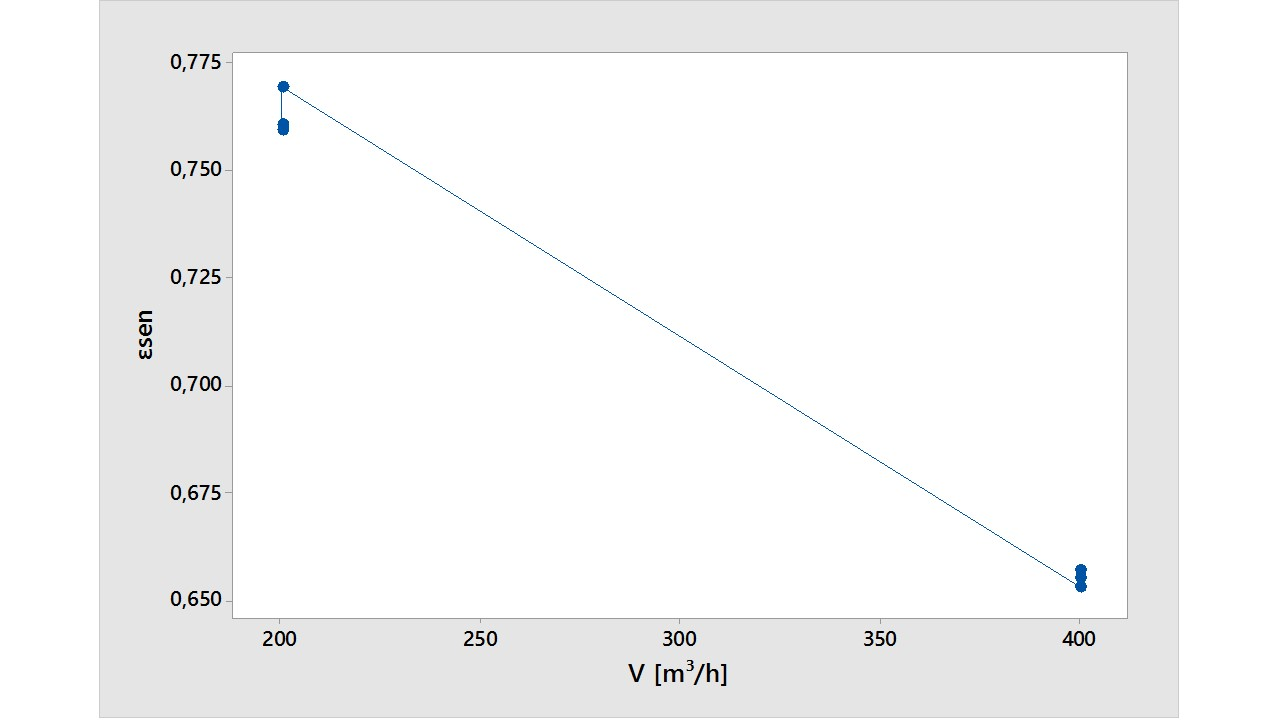
\includegraphics[width=0.98\textwidth]{pictures/Einfluss_Volumenstrom_sensible_Effektivitaet.jpg}
	\caption{sensible Effektivität über Volumenstrom}
	\label{Einfluss_Volumenstrom_sensible_Effektivitaet}
\end{figure}

Einfluss der Stromführung auf das Temperaturprofil
Der Einfluss der Stromführungsgeometrie ist dadurch bestimmt, dass sich Effekte, die aus Kreuzstromübertragern bekannt sind mit Effekten die aus Gegenstromübertragern bekannt sind überlagern.

Bei einem reinen adiabten Gegenstromübertrager ist die Temperatur über die $\alpha$- und $\beta$- Achse konstant. Die Temperatur ändert sich entlang der Strömungsachse. Abbildung … zeigt eine vereinfachte Darstellung des Temperaturverlaufes in einem Gegenstromübertrager entlang der Strömungsrichtung. Die Temperaturverläufe wurden vereinfacht linear angenommen. Der Wärmekapazitätskoeffizient ist auf der Feedseite und der Sweepseite gleich groß. Daher besitzen beide Geraden die gleiche Steigung.

%Abbildungen zum reinen Gegenstromübertragung

Da sich die kälteste Stelle des Frischluftstromes (Außenluft) mit der kältesten Stelle des Sweepstromes (Fortluft) trifft und die heißestes Stelle des Frischluftstromes mit der heißesten Stelle des Sweepstromes ist die Temperaturdifferenz zwischen beiden Strömen konstant. So kann das Potential des Sweepstromes optimal ausgenutzt werden. 

Für einen reinen Kreuzstromübertrager gilt dies nicht. Wie Abblidung …. zeigt, treffen in einer Ecke des Kreuzstromübertragers die heißeste und die kälteste Stelle der Luftströme aufeinander. So kann der Volumenstrom der an einer Seite des Kreuzstomübertragers nicht das volle Potenzial der Temperaturdifferenz zwischen Außenluft und Abluft nutzen. Unter den gleichen Bedingungen wie der Betrachtung des reinen Gleichstromübertragers, entsteht das in der Abbildung ... dargestellte Temperaturprofil. 

%Abbildung zum reinen Kreuzübertrager

Dieser Effekt tritt in abgeschwächter Form auch bei dem vorliegenden Enthapieübertrager auf und nimmt so Einfluss auf das entstehende Temperaturprofil in $\alpha$ - Richtung.




Um die Einflüsse der anderen drei Faktoren abschätzen zu können, wurde ein Kreuz aus Temperaturmesssensoren (PT100) direkt an den Austrittsflächen des Übertragers angebracht, wie in \ref{cha:Teil3} beschrieben


Anordnung

%Abbildung Kreuzanordnung

In Abbildung \ref{Temperaturprofil_ueber_der_Abstroemflaeche} ist das mittlere Temperaturprofil aus den Messungen 1-23 aus Tabelle--- über $\alpha$ und $\beta$ dargestellt. Dabei stellen $\alpha$ und $\beta$ die Koordinaten eines orthogonalen Koordinatensystems dar, das parallel zur jeweiligen Abströmfläche liegt. Sowohl für die Fortluft als auch für die Abluft ergibt sich eine Funktion zweiten oder höheren Grades.

\begin{figure} [h]
	\centering
	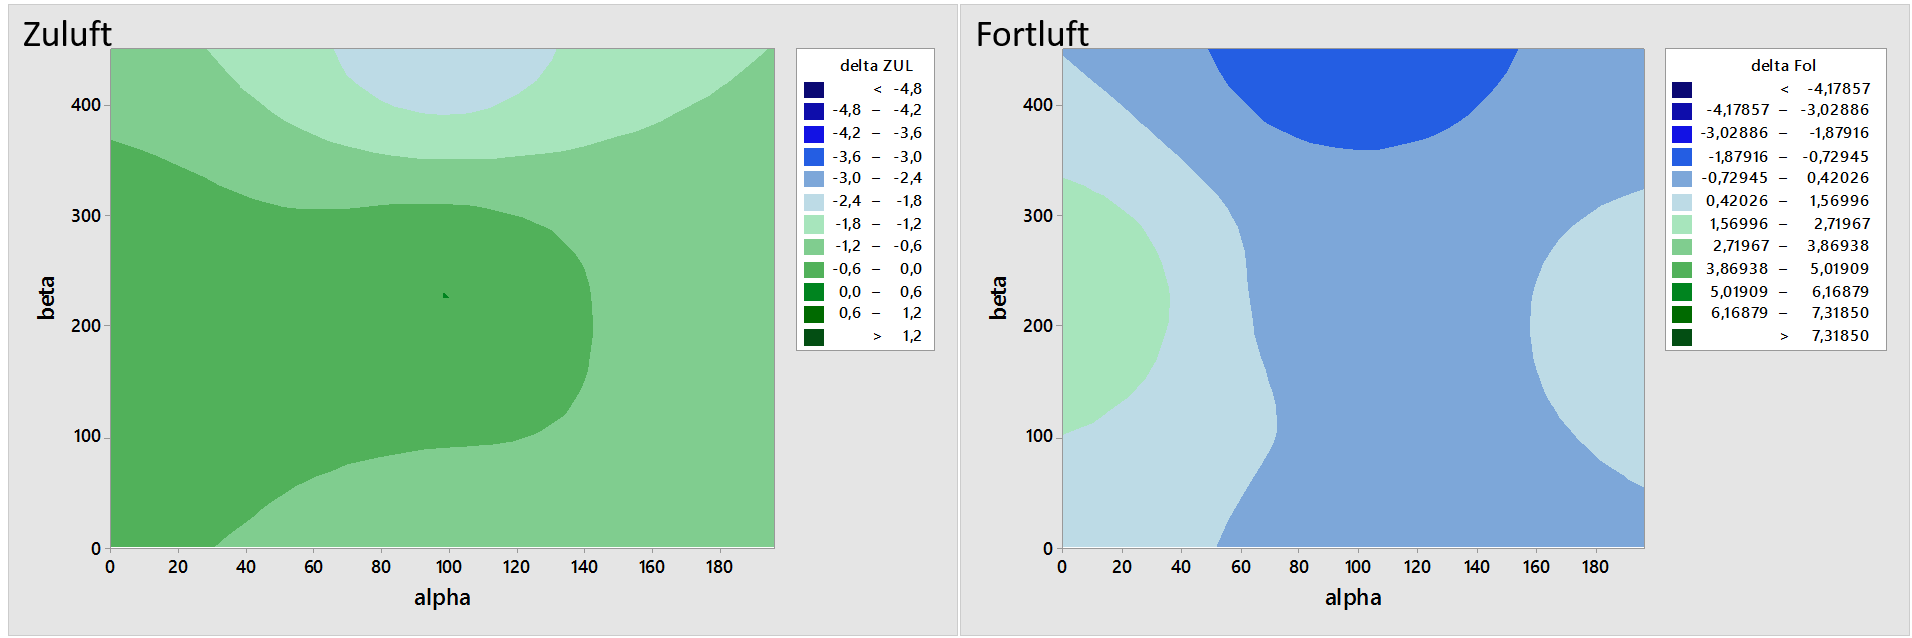
\includegraphics[width=0.98\textwidth]{pictures/Temperaturprofil_ueber_der_Abstroemflaeche.jpg}
	\caption{Temperaturprofil über der Abströmfläche}
	\label{Temperaturprofil_ueber_der_Abstroemflaeche}
\end{figure}


Um die Effekte über die einzelnen Achsen zu Betrachten, ist es Sinnvoll diese auch einzeln, also eindimensional darzustellen. Abbildung ... zeigt den Verlauf der Fortlufttemperatur und der Zulufttemperatur über $\alpha$.
Die Abbilung zeigt, dass die Temperatur auf der Zuluftseite und der Abluftseite bei $\alpha$ = 0 ihren höchsten Wert aufweist und entlang der $\alpha$ - Achse sinkt. Eine niedrige Temperatur auf der Fortluftseite wird durch einen hohen Übertragungsgrad hervorgerufen. Auf der Zuluftseite lässt eine hohe Temperatur auf eine hohen Übertragungsgrad schließen.

Abbildung ... zeigt die Anordnung der Luftströme zueinander und den Verlauf der $\alpha$ - Achse und der  $\beta$ - Achse. Die gemessenen Ergebnisse entsprechen den Erwartungen, die aus der Betrachtung eines Kreuzstromübertragers entstehen. Der Zuluftstrom passiert auf der  $\alpha$_{0} - Seite ($\alpha$ = 0) den noch heißen Abluftstrom. Die andere Seite des Zuluftstroms passiert den bereits abgekühlten Fortluftstrom. Entsprechend ist die  $\alpha$_{0} die heißere Seite
Der Fortluftstrom passiert auf der $\alpha$_{196} - Seite den noch kalten Außenluftstrom. Die  $\alpha$_{0} - Seite des Zuluftstroms passiert den bereits erwärmten Zuluftstrom. Entsprechend ist die  $\alpha$_{0} - Seite die heißere Seite.

Abbildung ... zeigt den Verlauf der Fortluft- und der Zulufttemperatur über die $\beta$ - Achse. Sowohl für in der Zuluft als auch für die Fortluft fällt die Temperatur über die $\beta$ - Achse, das heißt von unten nach oben. Dies lässt daraus schließen, dass die gemessenen Effekte nicht aus einem veränderten Übertragungsverhalten über die $\beta$ - Achse kommen. Möglich ist, dass sich hier eine Schichtung der Luft einstellt.
 
Mitteln der Fortluft- und Zulufttemperatur

Um Wärmeströme und somit auch die Übertragungsgrößen des Enthalpieübertragers errechnen zu können wird eine gemittelte Temperatur für den Zuluftstrom und für den Fortluftstrom benötigt.

Eine Möglichkeit die Temperatur zu mitteln besteht darin ein Regressionsmodell, wie in Abbildung \ref{Temperaturprofil_ueber_der_Abstroemflaeche} zu erzeugen. Eine Integration der Regressiongleichung über $\beta$ und $\alpha$ erzeugt ein Flächen Integral. Eine Division des errechneten Flächenintegrals $I_{TF}$ durch den Flächeninhalt A_{Abst} der Abströmfläche ergibt den gemittelten Wert der Zuluft- beziehungsweise der Ablufttemperatur. Der Flächeninhalt ergibt sich dabei aus
\begin{equation}
A_{Abst}= \beta*\alpha
\end{equation}

In für diese Arbeit ist dieses Vorgehen jedoch nicht sinnvoll. Die Regressionsgleichung muss in die Eckpunkte der Strömungsfläche interpoliert werden. Da die Temperaturverteilung an der Abströmfläche nicht eindeutig anhand physikalischer Gegebenheiten erklärt werden kann, sind die Regressionsgleichungen empirisch ermittelt. Entsprechend ist eine Verwendung zur Extrapolation nicht zweckmäßig. 

Bei Versuchen mit mehreren Messpunkten ist die Mittelung über eine Regressionanalyse jedoch gut einsetzbar. Dafür ist jedoch mindestens eine Belegung der Eckpunkte mit Messsensoren notwendig.

Alternativ wurde in dieser Arbeit die Abströmfläche in vier gleichgroße Teilbereiche zerlegt. Dabei fungieren die Mittellinie entlang der $\beta$-Achse ($\alpha = 98$) und die Mittellinie entlang der $alpha$-Achse ($\beta = 225$) als Trennlinien. Für jeden Teilbereich wird jeweils die Mittelpunkttemperatur des Bereichs ermittelt. Dazu wird jeweils eine lineare Verlauf entlang der  $\beta$-Achse und entlang der  $\alpha$-Achse angenommen. Über die drei jeweils angrenzend gemessenen Temperaturen ergibt sich die Temperatur des Bereichs oben links $T_{OL}$ zu 
\begin{equation}
T_{OL} = ((T_{FOL-L}-T_{FOL-Mitte})*\frac{125}{250}+(T_{FOL-O}-T_{FOL-Mitte})*\frac{50}{100})+T_{FOL-Mitte},
\end{equation}

die Temperatur des Bereichs oben rechts $T_{OR}$ zu
\begin{equation}
T_{OR} = ((T_{FOL-R}-T_{FOL-Mitte})*\frac{125}{250}+(T_{FOL-O}-T_{FOL-Mitte})*\frac{50}{100})+T_{FOL-Mitte},
\end{equation}

die Temperatur des Bereichs unten links $T_{UL}$ zu
\begin{equation}
T_{UL} = ((T_{FOL-L}-T_{FOL-Mitte})*\frac{125}{250}+(T_{FOL-U}-T_{FOL-Mitte})*\frac{50}{100})+T_{FOL-Mitte}
\end{equation}

und die Temperatur des Bereichs unten rechts $T_{OR}$ zu
\begin{equation}
T_{UR} = ((T_{FOL-R}-T_{FOL-Mitte})*\frac{125}{250}+(T_{FOL-U}-T_{FOL-Mitte})*\frac{50}{100})+T_{FOL-Mitte}.
\end{equation}



Aus den vier gemittelten Teilflächen wird die gesamte Mitteltemperatur $T_{FOL}$ aus dem arithmetischen Mittel  
\begin{equation}
T_{FOL} = \frac{T_{OL}+T_{OR}+T_{UL}+T_{UR}}{4}
\end{equation}
gebildet. 
Die Rechnung für die Zulufttemperatur $T_{ZUL}$ erfolgt analog.







